\begin{figure}[h!]
    \centering
    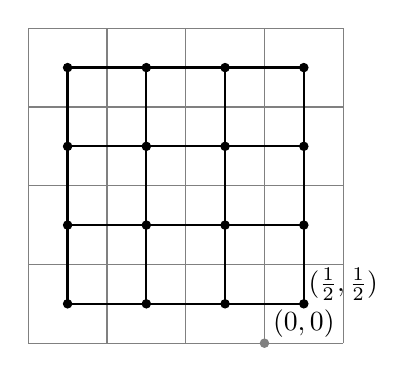
\begin{tikzpicture}
        % Z^2
        \foreach \x in {0, 1, ..., 4} {
            \draw[gray] (0, \x) -- (4, \x);
            \draw[gray] (\x, 0) -- (\x, 4);
        }
        
        % Z^2 dual
        \foreach \i in {0.5, 1.5, ..., 3.5} {
            \draw[black, thick] (0.5, \i) -- (3.5, \i);
            \draw[black, thick] (\i, 0.5) -- (\i, 3.5);
            \foreach \j in {0.5, 1.5, ..., 3.5} {
                \filldraw[black] (\i, \j) circle (1.5pt);
            }
        }
        
        \filldraw[gray] (3.0, 0.0) circle (1.5pt); 
        
        \node at (3.5, 0.25) {$(0, 0)$};
        \node at (4.0, 0.75) {$(\frac{1}{2}, \frac{1}{2})$};
                
    \end{tikzpicture}
    \caption{A $5 \times 5$ section of the square lattice and its dual}
    \label{fig:dual}
\end{figure}